\documentclass[11pt,a4paper]{article}

\usepackage[brazil]{babel}
\usepackage[T1]{fontenc}
\usepackage[latin1]{inputenc}
\usepackage{amsmath,amsfonts}
\usepackage{bussproofs}
\usepackage{amssymb}
\usepackage{tikz}
\usepackage{latexsym}
\usepackage{pgf}
 
\begin{document}

\section{Divers\~ao com Eletr\^onica Anal\'ogica}



Resistores s\~ao componentes el\'etricos / eletr\^onicos muito utilizados para redu\c{c}\~ao de corrente em circuitos.
A medida do quanto de resist\^encia possui um resitor \'e medida em Ohms ($\Omega$) e este valor \'e usualmente
descrito usando um c\'odigo formado por cores. As duas primeiras cores do c\'odigo representam os dois d\'igitos mais
significativos do valor, a terceira cor representa uma pot\^encia de 10.

A tabela seguinte apresenta o significado de cada uma das cores em suas respectivas posi\c{c}\~oes:
	      \begin{center}
              \begin{tabular}{|c|c|c|c|}
                  \hline
		  Cor      & $1^{a}$ pos. & $2^{a}$ pos. & $3^{a}$ pos. (Mult.)\\\hline
                  Preto    & $0$          &  $0$         & $ 10^{0}$      \\\hline
                  Marrom   & $1$          &  $1$         & $ 10^{1}$      \\\hline
                  Vermelho & $2$          &  $2$         & $ 10^{2}$      \\\hline
                  Laranja  & $3$          &  $3$         & $ 10^{3}$      \\\hline
                  Amarelo  & $4$          &  $4$         & $ 10^{4}$      \\\hline
                  Verde    & $5$          &  $5$         & $ 10^{5}$      \\\hline
                  Azul     & $6$          &  $6$         & $ 10^{6}$      \\\hline
                  Violeta  & $7$          &  $7$         & $ 10^{7}$      \\\hline
                  Cinza    & $8$          &  $8$         & $ 10^{8}$      \\\hline
                  Branco   & $9$          &  $9$         & $ 10^{9}$      \\\hline
                  Ouro     & -            &   -          & $ 10^{-1}$     \\\hline
                  Prata    & -            &   -          & $ 10^{-2}$     \\\hline
              \end{tabular}
              \end{center}
Como exemplo, considere o seguinte c\'odigo: Verde-Azul-Amarelo. Como as duas primeiras cores s\~ao Verde e Azul,
temos que os dois d\'igitos mais significativos deste resistor s\~ao: 5 e 6. O multiplicador (terceira cor) deve 
ser $10^{4}$. 

Desta maneira, temos que o resistor de c\'odigo  Verde-Azul-Amarelo possui uma resist\^encia
de $56\times 10^{4}\Omega$.

Considere o seguinte tipo de dados Haskell, que representa as cores utilizadas para codificar valores de resist\^encia:
\begin{verbatim}
data Color = Black | Brown | Red | Orange | Yellow | Green 
           | Blue | Violet | Gray | Gold | Silver
           deriving (Eq, Ord)
\end{verbatim}

e a seguinte tabela que representa os poss\'iveis valores associados a cada cor:

\begin{verbatim}
type Table = [(Color, [Maybe Float])]

table :: Table
table = [(Black,  [Just 0.0, Just 0.0, Just 0.0]),
         (Brown,  [Just 1.0, Just 1.0, Just 10.0]),
         (Red,    [Just 2.0, Just 2.0, Just 100.0]),
         (Orange, [Just 3.0, Just 3.0, Just 1000.0]),
         (Yellow, [Just 4.0, Just 4.0, Just 10000.0]),
         (Green,  [Just 5.0, Just 5.0, Just 100000.0]),
         (Blue,   [Just 6.0, Just 6.0, Just 1000000.0]),
         (Violet, [Just 7.0, Just 7.0, Just 100000000.0]),
         (Gray,   [Just 8.0, Just 8.0, Just 1000000000.0]),
         (Gold,   [Nothing,  Nothing, Just 0,1]),
         (Silver, [Nothing,  Nothing, Just 0,01])]
\end{verbatim}
Observe que o valor \texttt{table} \'e uma lista de pares formados por um valor de tipo \texttt{Color} e 
uma lista de valores de tipo \texttt{Maybe Float}, onde uma posi\c{c}\~ao da lista representa uma determinada coluna na tabela. Por exemplo,
a cor vermelho (representada pelo valor \texttt{Red}) possui como valores associados \`a primeira, segunda e terceira coluna os n\'umeros $2$, $2$ e
$10^{2}$ respectivamente e isto \'e representado no valor \texttt{table} pelo par \texttt{(Red,    [Just 2.0, Just 2.0, Just 100.0])}. Quando um 
determinado valor n\~ao est\'a presente na tabela, este \'e representado por \texttt{Nothing}.

Com base no anteriormente apresentado, desenvolva o que se pede:

\begin{enumerate}

    \item Desenvolva a fun\c{c}\~ao
    \begin{center}
        \texttt{value :: Color -> Int -> Maybe Float}
    \end{center}    
    que recebe como par\^ametros uma cor e um n\'umero inteiro correspondente ao n\'umero de uma coluna da tabela de valores de cores e retorna
    o valor associado \`a cor e a respectiva posi\c{c}\~ao desta na tabela. Caso o n\'umero da coluna seja inv\'alido (menor que $0$ ou maior que $3$),
    sua fun\c{c}\~ao deve retornar como resultado o valor \texttt{Nothing}.
    \item Considere agora, o seguinte tipo de dados que representa um resistor:
    \begin{center}
       \texttt{data Resistor = Resistor [Color] deriving (Eq, Ord)}
    \end{center}
    Um resistor de c\'odigo Vermelho-Marrom-Amarelo seria representado pelo seguinte valor:
    \begin{center}
       \texttt{Resistor [Red, Brown, Yellow]}
    \end{center}
    \begin{enumerate}
	\item A representa\c{c}\~ao de resistores utilizando o tipo \texttt{Resistor} permite que um resitor seja constru\'ido utilizando um 
              n\'umero arbitr\'ario de cores, o que \'e incorreto, j\'a que o c\'odigo de cores \'e formado apenas por tr\^es posi\c{c}\~oes.
              Desenvolva a fun\c{c}\~ao
              \begin{center}
                   \texttt{valid :: Resistor -> Bool}
              \end{center}
              que retorna verdadeiro se o resistor fornecido como par\^ametro possui $3$ e somente $3$ cores.
        \item Utilizando a fun\c{c}\~ao \texttt{value} definida por voc\^e no exerc\'icio 1, defina a fun\c{c}\~ao:
              \begin{center}
                   \texttt{resistence :: Resistor -> Float}
              \end{center}
              que calcula o valor num\'erico do c\'odigo de cores deste resistor. Como exemplo considere:
              \begin{center}
		   \texttt{resistence (Resistor [Red, Brown, Yellow]) = 210000.0}
              \end{center}
    \end{enumerate}
    \item Resistores s\~ao mais \'uteis quando unidos para formar circuitos. Considere o seguinte tipo de dados que representa 
          circuitos:
\begin{verbatim}
data Circuit = Parallel Circuit Circuit
             | Series   Circuit Circuit
             | Single Resistor
             deriving (Eq, Ord)
\end{verbatim}	
Onde o construtor \texttt{Single} representa um circuito formado por apenas um resistor, o construtor \texttt{Series} representa dois circuitos de
resistores em s\'erie e o construtor \texttt{Parallel} representa dois circuitos de resistores em paralelo. As figuras 1 e 2 apresentam circuitos
em s\'erie e paralelo formados por tr\^es resistores \texttt{R1}, \texttt{R2} e \texttt{R3}.
\begin{figure}[htp]			
    \centering
    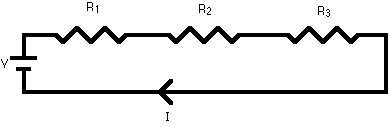
\includegraphics[scale=0.4]{Rseries.jpg}
    \caption{Circuito de resistores em s\'erie}
\end{figure}
\begin{figure}[htp]			
    \centering
    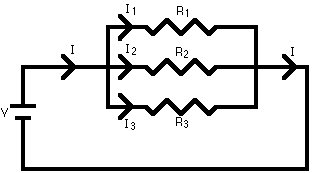
\includegraphics[scale=0.4]{Rparallel.jpg}
    \caption{Circuito de resistores em paralelo}
\end{figure}
Supondo que \texttt{r1}, \texttt{r2} e \texttt{r3} sejam valores do tipo \texttt{Resistor}, os circuitos apresentados nas figuras 1 e 2 podem
ser representados pelos seguintes valores do tipo \texttt{Circuit}, respectivamente.
\begin{verbatim}
circuit1 = Series (Series (Single r1) (Single r2))
                  (Single r3)

circuit2 = Parallel (Parallel (Single r1) (Single r2))
                    (Single r3)
\end{verbatim}
\begin{enumerate}
   \item Considerando, que \texttt{r1}, \texttt{r2}, \texttt{r3} e \texttt{r4} s\~ao valores do tipo resistor previamente definidos, 
        defina o circuito formado por estes resistores que est\'a representado na figura 3 utilizando um valor do tipo \texttt{Circuit}:
\begin{figure}[htp]			
    \centering
    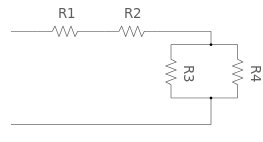
\includegraphics[scale=0.5]{circuit.jpg}
    \caption{Circuito de resistores}
\end{figure}         
   \item Um circuito representado por um valor do tipo \texttt{Circuit} \'e dito ser v\'alido se e somente se cada um dos resistores que o comp\~oe
         \'e v\'alido, isto \'e, possui um c\'odigo de cores correto. Utilizando a fun\c{c}\~ao \texttt{valid :: Resistor -> Bool}, implementada por 
         voc\^e no item 2-a), desenvolva a fun\c{c}\~ao:
         \begin{center}
            \texttt{validCircuit :: Circuit -> Bool}
         \end{center}
         que retorna verdadeiro se o valor do tipo \texttt{Circuit} fornecido como par\^ametro for formado apenas por resistores v\'alidos e falso
         caso contr\'ario.
   \item \'E fato sabido que a resist\^encia equivalente de um circuito formado por $n$ resistores em s\'erie pode ser obtida pela seguinte f\'ormula:
         \begin{center}
         $r_{eq} = \sum_{i=1}^{n}r_{i}$
         \end{center}
         onde $r_{i}$ \'e o valor em Ohms da resist\^encia do i-\'esimo resistor deste circuito em s\'erie. Para circuitos formados por $n$ resistores
         em paralelo temos que a resist\^encia equivalente deste circuito \'e dada pela seguinte f\'ormula:
         \begin{center}
             $\frac{1}{r_{eq}} = \sum_{i=1}^{n}\frac{1}{r_{i}}$
         \end{center}
         Com base no apresentado, implemente a fun\c{c}\~ao
         \begin{center}
	     \texttt{circuitResistence :: Circuit -> Float}
         \end{center}
         que calcula a resist\^encia equivalente de um circuito utilizando as f\'ormulas anteriormente apresentadas e a fun\c{c}\~ao \texttt{resistence},
         definida no item 2-c). \textit{Dica:} Para calcular o inverso de $n$, isto \'e, $\frac{1}{n}$, utilize a fun\c{c}\~ao \texttt{recip} (j\'a 
         definida na biblioteca da linguagem). Para qualquer valor num\'erico \texttt{n}, \texttt{recip n} = $\frac{1}{n}$.
\end{enumerate}
\end{enumerate}
\end{center}
\end{enumerate}
\end{document}
